% BANKS-SOURCE: pdf=149 print=139 kind=section id=9.1
\subsection{Divergences in Feynman graphs}

% BANKS-SOURCE: pdf=149 print=139 kind=prose
continuation of the Euclidean propagator. Integrating out degrees of freedom
is always done in the Euclidean path integral.

The effective equations of motion for $x(t)$ are non-local, but if we are
interested only in time scales much longer than $\Omega^{-1}$ we can make the
expansion
\[
  G\simeq\frac{1}{\Omega^2}\delta(t-s)
  -\frac{1}{\Omega^4}\partial_t^2\delta(t-s)+\cdots .
\]
We get an infinite series of higher-derivative terms in the approximately
local equations for $x$. When the solution for $x$ contains only frequencies
$\omega_i\ll\Omega$, the higher-order terms in the series are negligible, and
we refer to them as \emph{irrelevant}.

To begin our consideration of ultraviolet divergences, we study the $\phi^n$
scalar field theory. A 1PI Feynman graph with $E$ external legs and $V$
vertices has $I=(nV-E)/2$ internal lines. The number of loop integrals is
\[
  L=I-V+1=1+\frac{(n-2)V-E}{2} .
\]
We evaluate the graphs in momentum space and look at the region of integration
where all loop momenta are large. Then we can drop all masses and external
momenta in the internal propagators. In this regime, the integral looks like
\[
  \int\frac{\dd^{D L}p}{p^{2I}},
\]
and it diverges if $D L\geq2I$. In terms of $V$ and $E$, this inequality is
\[
  D+\frac{D}{2}((n-2)V-E)\geq nV-E,
\]
or, equivalently,
\[
  2D\geq\bigl(2n-D(n-2)\bigr)V+(D-2)E .
\]
For $D=4$ this reduces to $4\geq(4-n)V+E$. The usual classification then
follows: for $n=3$, only a finite number of orders of perturbation theory will
have such a divergence; for $n=4$, the degree of divergence is independent of
the order; for $n>4$, it increases with the order. At fixed perturbative order,
the degree decreases with the number of external legs, and each external-momentum
derivative lowers it by one.

% BANKS-SOURCE: pdf=150 print=140 kind=prose
Indeed, all of these facts are a simple consequence of dimensional analysis,
and the fact that masses on internal lines are negligible in the high-momentum
regime.\footnote[1]{This is not true for the masses of massive gauge bosons in
unitary gauges. As a consequence of this fact, the unitary gauge Lagrangians
are in fact non-renormalizable as quantum field theories of Green functions.
However, one can show that the S-matrix in these theories is identical to that
of the physical particles of the $R_\kappa$-gauge Lagrangian, which is
renormalizable. From the point of view of the $R_\kappa$ gauge the
non-renormalizable divergences of Green functions of unitary gauge fields
arise because these are really gauge-invariant non-polynomial functions of the
$R_\kappa$ gauge fields.}
\BanksImplicitHook{I-CH09-003}
The coupling $\lambda_n$ of a $\phi^n$ interaction has mass dimension
$D-n(D-2)/2$. A connected $E$-point function of scalar fields has mass
dimension $E(D-2)/2$, and its stripped Fourier transform has dimension
$D-E(D+2)/2$ if we leave off the momentum-conservation delta function. An
$E$-point 1PI function thus has dimension $D-E(D-2)/2$. The overall number of powers of momentum in the Feynman
graph integrals is thus completely determined by dimensional analysis. An
interaction with positive (negative) mass dimension will have fewer and fewer
(more and more) divergent integrals as we go to higher and higher order. We
call interactions of positive mass dimension \emph{super-renormalizable},
those of negative dimension, \emph{non-renormalizable}, and those of dimension
0, simply \emph{renormalizable}. For reasons that will become apparent later,
these terms are often replaced by \emph{relevant}, \emph{irrelevant}, and
\emph{marginal}.

In purely mechanical terms, the basic idea of renormalization is that, at any
order in perturbation theory, the divergences all reside in a finite number of
$E$-point functions, and are polynomial functions of momenta. The latter
remark follows from the fact that, if we take a finite number of derivatives of
the Feynman graph, then the superficial divergences go away, because we have
introduced more internal propagators. As a consequence, we can find local
interactions of the form
$c_n(\lambda_n)^V\partial^{a_1}\phi\ldots\partial^{a_E}\phi$, which,
when added to the theory, can subtract away all of the divergences. In order
to do this, we must choose the coefficients $c_n$ to be infinite. A more
sensible mathematical procedure would be to define a cut-off theory, which
effectively gets rid of the divergences above some high scale $\Lambda$, and
allow the $c_n$ to depend on $\Lambda$ in such a way that the limit
$\Lambda\to\infty$ exists.

It is not clear that this simple subtraction procedure actually works, for we
have dealt only with the region of integration where all momenta are large. A
1PI Feynman graph contains many 1PI sub-graphs. Even if the overall degree of
divergence of the graph is negative, we might have a sub-graph whose integrals
diverge when all other momenta in the graph are held fixed. The second key idea
of perturbative renormalization theory is that ``sub-divergences have already
been taken care of by subtractions at lower orders in perturbation theory.''
This is far from clear in purely graphical terms. To understand why it is
true (still in a purely mechanical sense) we will return to the coordinate-space
definition of Feynman graphs.

% BANKS-SOURCE: pdf=150 print=140 kind=prose
Divergent loop integrals fall into two distinct classes. The first is
associated with loops that consist of a single propagator attached to the same
vertex (ear diagrams), Figure~\ref{fig:9.1}(a). The second consists of loops
that include several vertices like Figure~\ref{fig:9.1}(b). Both can be
understood in terms of the singularities in operator products in free-field
theory. Indeed, interactions like $\phi^n$ are not well-defined operators in
the free-field theory. Wick's

% BANKS-SOURCE: pdf=151 print=141 kind=page-boundary
% BANKS-SOURCE: pdf=151 print=141 kind=figure id=9.1
\begin{figure}[htbp]
  \centering
  % BANKS-SOURCE: pdf=151 print=141 kind=figure id=9.1
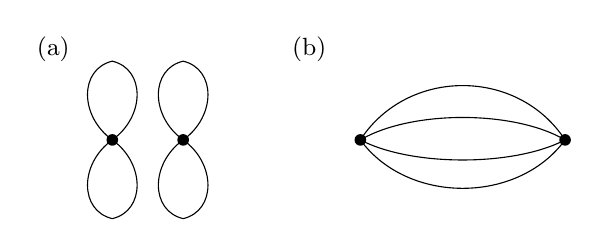
\begin{tikzpicture}[x=1cm,y=1cm,line cap=round,line join=round,
  every node/.style={font=\small}]
  % (a) Two "ear" diagrams: each is a single vertex carrying two
  % self-contractions, drawn as a vertical figure-eight.
  \node at (-2.95,1.15) {(a)};
  \foreach \cx in {-2.20,-1.30} {
    % upper ear
    \draw (\cx,0) .. controls (\cx-0.42,0.30) and (\cx-0.42,0.90)
      .. (\cx,1.00)
      .. controls (\cx+0.42,0.90) and (\cx+0.42,0.30) .. (\cx,0);
    % lower ear
    \draw (\cx,0) .. controls (\cx-0.42,-0.30) and (\cx-0.42,-0.90)
      .. (\cx,-1.00)
      .. controls (\cx+0.42,-0.90) and (\cx+0.42,-0.30) .. (\cx,0);
    \fill (\cx,0) circle (2.1pt);
  }
  % (b) Two vertices joined by four internal lines.
  \node at (0.30,1.15) {(b)};
  \fill (0.95,0) circle (2.1pt);
  \fill (3.55,0) circle (2.1pt);
  \draw (0.95,0) .. controls (1.55,0.92) and (2.95,0.92) .. (3.55,0);
  \draw (0.95,0) .. controls (1.60,0.38) and (2.90,0.38) .. (3.55,0);
  \draw (0.95,0) .. controls (1.60,-0.34) and (2.90,-0.34) .. (3.55,0);
  \draw (0.95,0) .. controls (1.55,-0.82) and (2.95,-0.82) .. (3.55,0);
\end{tikzpicture}

  \caption{Examples of divergent diagrams.}
  \label{fig:9.1}
\end{figure}

% BANKS-SOURCE: pdf=151 print=141 kind=prose
theorem shows us that products of operators at different points diverge as the
points are taken to coincide. This leads to the idea of an \emph{operator
product expansion} (OPE):
\[
  \phi(x)\phi(y)=\sum_N C_N(x-y)O_N(y) .
\]
In free, massless field theory, dimensional analysis shows us that, if the
operator $O_N$ has mass dimension $d_N$, then
$C_N(x)\sim |x|^{-D+2+d_N}$. These operators are called
$:\!\phi\,\partial^{\mu_1}\ldots\partial^{\mu_{N-2}}\phi\!:$, the normal
ordered product of $\phi$ with its partial derivatives. The function $C_{N-2}$
has the tensor transformation properties to make the OPE Lorentz covariant.
Notice that $O_0$, the identity operator, also appears in the list. It is the
only one with a divergent coefficient. However, we can now go on to consider
higher-order powers of $\phi$ and its derivatives. The result is an infinite
collection of finite operators, which we will again label $O_N$. There are now
many ways to get an operator with a given mass dimension. The generalized OPE
has the form
\[
  O_N(x)O_M(y)=\sum_K C_{NM}^{\;K}(x-y)O_K(y),
\]
where we have again suppressed the tensor properties of operators and their
coefficient functions. The c-number functions in the OPE are called Wilson
coefficients. $C_{NM}^{\;K}$ scales like
$x^{-d_N-d_M+d_K}$. Wick's theorem guarantees that these are in fact operator
relations. That is, the behavior of an $n$-point Green function when $k$ of
the points are taken together is universal, and can be written as singular
coefficients depending on the coinciding points, multiplied by a function of
the coincident point and the other $n-k$ points in the function.

In general, we see that, even after we have defined finite operators $O_N$,
their products when points are taken together will often diverge. Now consider
the application of all of this to the perturbation expansion. The series
corresponds to integrals over interaction vertices, defined as naive powers of
the field at the same point. We can expect divergences corresponding to
``improper normal ordering'' (the correct definition of local composite
operators) as well as to singular products of normal ordered operators (since
we must integrate over coinciding interaction points). The former correspond
to ``ear'' diagrams. They can be understood by writing out $\phi^n$ in terms
of normal ordered operators and subtracting the divergent terms.

The OPE allows us to understand and deal with the coinciding point divergences
in a similar way. We have to evaluate
\[
  \int\left\langle:\!\phi^n(x_1)\!:\ldots:\!\phi^n(x_k)\!:\right\rangle .
\]
Near coinciding points, we can use the OPE to write this in terms of Wilson
coefficients and finite operators. This tells us that we can always subtract
away the divergences by

% BANKS-SOURCE: pdf=152 print=142 kind=page-boundary
adding local operators to the Lagrangian. Furthermore, the sub-divergences that
occur at order $k$, when $p<k$ points coincide, will have precisely the form of
the Lagrangian we subtracted at order $p$ when this particular divergence first
showed up.

So we have understood, at least in a hand-waving and mechanical way, how it is
that divergences in the field-theoretic perturbation expansion can be absorbed
into (formally infinite) redefinitions of the Lagrangian. We can also see that
the structure of these subtractions will be quite different for irrelevant
perturbations, versus marginal or relevant ones. For irrelevant perturbations,
we will generate every interaction consistent with the symmetries of the
problem, if we go to high enough order of perturbation theory. For relevant or
marginal interactions, the subtraction process stops with a finite set of
operators. This means that irrelevant interactions have no (cut-off-independent)
meaning. When we add an infinite counterterm to subtract a
divergence, we have no rule to tell us how much of a finite coefficient one
should add to the infinite one. Thus, theories with irrelevant interactions
seem to make no predictions at all. Later we will see that this judgement is a
bit too harsh, but that will have to wait until we understand the meaning of
renormalization, not just its mechanics.

I want to end this section by noting that the definition of normal ordered
operators is ambiguous in massive free-field theory. The Wilson coefficients
are no longer required to be pure power laws. Indeed, the massless Wilson
coefficients are multiplied by functions of $m|x-y|$, which are non-singular as
$m|x-y|$ goes to zero. As a consequence, it is impossible to identify a
normal ordered operator as the coefficient of a certain power of $|x-y|$ in
the short-distance expansion. There is an ambiguity because we can replace an
operator of a given mass dimension by a polynomial in $m$, with higher powers
of $m$ multiplying operators that would have lower mass dimension in the
massless theory. A standard definition of normal ordered products is to
reorder the creation and annihilation operators so that all creation operators
stand to the left of all annihilation operators. This is in fact the origin of
the name normal ordered operator. We should remember that this is just an
arbitrary convention. It is an example of what we will call a
\emph{renormalization-scheme ambiguity} in the general theory of
renormalization.
